\chapter{EXTRAÇÃO DE PONTOS DE FORMA AUTOMÁTICA} \label{cha:processamento-imagem} 

Neste capítulo, será apresentado o método de extração automática de pontos de forma a facilitar a modelagem de \textit{splines} para reconhecimento facial. O método proposto consiste em um algoritmo que utiliza técnicas de processamento de imagem e otimização para extrair pontos relevantes em imagens faciais. A abordagem é baseada na detecção de características faciais, seguida pela extração de contornos e filtragem dos pontos obtidos.

Inicialmente, realizamos uma pesquisa para identificar as principais características faciais a serem extraídas, decidindo focar na detecção dos olhos, nariz e boca. Para isso, utilizamos o algoritmo Haar Cascade para detectar o rosto da pessoa na imagem, concentrando a análise nessa área específica e facilitando a detecção das características menores \cite{BoostedCascade}.

Em seguida, utilizamos o método \texttt{Canny} do OpenCV \cite{CannyAplicacao} para extrair os contornos das características faciais. O \texttt{Canny} é um algoritmo de detecção de contornos eficiente que nos ajuda a identificar os limites das características faciais com maior precisão \cite{Canny}.

Após a extração dos contornos, suprimimos alguns pontos fazendo o uso de grafos e árvores geradoras mínimas. Essa etapa é crucial para reduzir a quantidade de pontos a serem utilizados na modelagem das \textit{splines}, mantendo apenas os pontos mais significativos que representam as características faciais. A simplificação dos pontos é realizada utilizando o algoritmo construído de forma autoral e implementado em Python, que utiliza a biblioteca \textit{Scipy} \cite{Scipy} para encontrar a árvore geradora mínima. Essa abordagem garante que os pontos extraídos sejam representativos e relevantes para a modelagem das \textit{splines}.

Por fim, ainda é possível aplicar um filtro de suavização para diminuir a quantidade de pontos, fazendo isso de forma completamente aleatória, mantendo apenas os pontos iniciais e finais de cada segmento, o que pode ser útil para melhorar a qualidade da modelagem das \textit{splines}.

\section{MODELOS PARA DETECÇÃO DE CARACTERÍSTICAS}

Foi utilizada uma abordagem popular de detecção chamada Haar Cascade, implementada com OpenCV e Python. Este método, introduzido e estudado no artigo \cite{BoostedCascade}, permite a detecção eficaz das características faciais.

O classificador Haar Cascade já foi calibrado e validado com um vasto conjunto de dados de rostos humanos, eliminando a necessidade de calibração adicional. Basta carregar o classificador da biblioteca e utilizá-lo para detectar rostos em uma imagem de entrada.

Para distinguir com precisão entre amostras que contêm ou não um rosto humano, utilizamos um classificador forte, resultante da combinação de diversos classificadores. Esta técnica envolve a utilização de uma cascata de classificadores para identificar diferentes características em uma imagem.

Os seguintes classificadores foram utilizados:

\begin{itemize}
    \item \texttt{haarcascade\_frontalface\_default.xml}
    \item \texttt{haarcascade\_eye.xml}
    \item \texttt{haarcascade\_mcs\_nose.xml}
    \item \texttt{haarcascade\_mcs\_mouth.xml}
\end{itemize}

Todos os classificadores mencionados podem ser encontrados no repositório do OpenCV no GitHub \cite{HaarAplicacao}.

\subsection{Parâmetros}

Após carregar os classificadores, podemos utilizá-los aplicando quatro parâmetros específicos para cada um.

O método \texttt{detectMultiScale()} é utilizado para identificar faces de diferentes tamanhos na imagem de entrada. Os quatro parâmetros principais deste método são detalhados a seguir:

\begin{itemize}
    \item \textbf{\texttt{image}}:
    \begin{itemize}
    \item O primeiro parâmetro é a imagem em tons de cinza. Essa imagem serve como entrada para o método e com ela em tons de cinza facilita a detecção de características faciais.
    \end{itemize}

\item \textbf{\texttt{scaleFactor}}:
\begin{itemize}
    \item Este parâmetro é usado para reduzir o tamanho da imagem de entrada, facilitando a detecção de faces maiores pelo algoritmo. Especificamos um fator de escala de 1.1, indicando que queremos reduzir o tamanho da imagem em 10\%.
    \end{itemize}

\item \textbf{\texttt{minNeighbors}}:
\begin{itemize}
    \item O classificador em cascata aplica uma janela deslizante através da imagem para detectar faces. Essas janelas são representadas como retângulos. Inicialmente, o classificador captura um grande número de falsos positivos. O parâmetro \texttt{minNeighbors} especifica o número de retângulos vizinhos que precisam ser identificados para que um objeto seja considerado uma detecção válida, ou seja, valores pequenos como 0 ou 1 resultam em muitos falsos positivos, enquanto valores grandes podem levar à perda de verdadeiros positivos. É necessário encontrar um equilíbrio que elimine falsos positivos e identifique com precisão os verdadeiros positivos.
\end{itemize}

\item \textbf{\texttt{minSize}}:
\begin{itemize}
    \item Este parâmetro define o tamanho mínimo do objeto a ser detectado. O modelo ignorará faces menores do que o tamanho mínimo especificado.
\end{itemize}

\end{itemize}

Foi colocado como default para todos os classificadores os seguintes valores: 

{\small \texttt{detectMultiScale(image, scaleFactor=1.1, minNeighbors=5, minSize=(40, 50))}}

\subsection{Resultado da Detecção das Características}

Para realizar a detecção das características faciais, inicialmente identificamos o rosto na imagem. Este processo retorna um \textit{array} com quatro valores: as coordenadas $x$ e $y$ do ponto onde o rosto foi detectado, além de sua largura e altura. Em seguida, recortamos a imagem nessa região, de modo a isolar a face da pessoa.

Com o rosto isolado, aplicamos classificadores específicos para detectar o nariz, a boca e os olhos.

Essa abordagem, que realiza a detecção passo a passo, garante maior precisão na identificação das características menores, pois concentra a análise na área previamente delimitada pelo rosto.

Considere a  \autoref{fig:deteccao-caracteristicas} , onde a detecção das características faciais é realizada:

\begin{enumerate}
\item \textbf{Detecção do Rosto:} Para identificar e isolar o rosto na imagem usamos o classificador \texttt{haarcascade\_frontalface\_default.xml}.
\item \textbf{Detecção dos Olhos:} Aplicamos o classificador \texttt{haarcascade\_eye.xml} para localizar os olhos dentro da área do rosto previamente detectada.
\item \textbf{Detecção do Nariz:} Utilizamos o classificador \texttt{haarcascade\_mcs\_nose.xml} para identificar o nariz na mesma área delimitada.
\item \textbf{Detecção da Boca:} Finalmente, aplicamos o classificador 

\texttt{haarcascade\_mcs\_mouth.xml} para localizar a boca.
\end{enumerate}

\begin{figure}[h!]
    \caption{DETECÇÕES.}
    \centering
    \begin{minipage}[b]{0.45\textwidth}
        \centering
        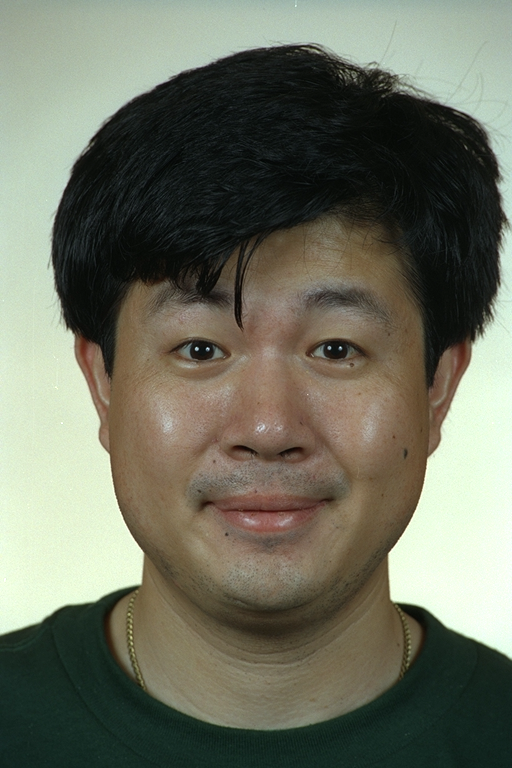
\includegraphics[width=0.9\linewidth]{fig/01_example_image.png}
        \legend{FONTE: \cite{FERET1,FERET2}}
        \label{fig:imagem}
    \end{minipage}
    \hfill
    \begin{minipage}[b]{0.45\textwidth}
        \centering
        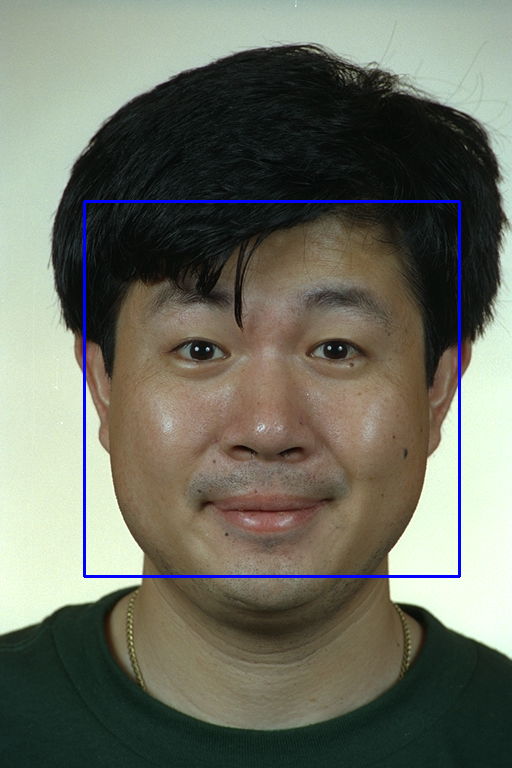
\includegraphics[width=0.9\linewidth]{fig/02_face.png}
        \legend{1º Detecção da face.}
        \label{fig:face}
    \end{minipage}

    \vspace{1cm}

    \begin{minipage}[b]{0.45\textwidth}
        \centering
        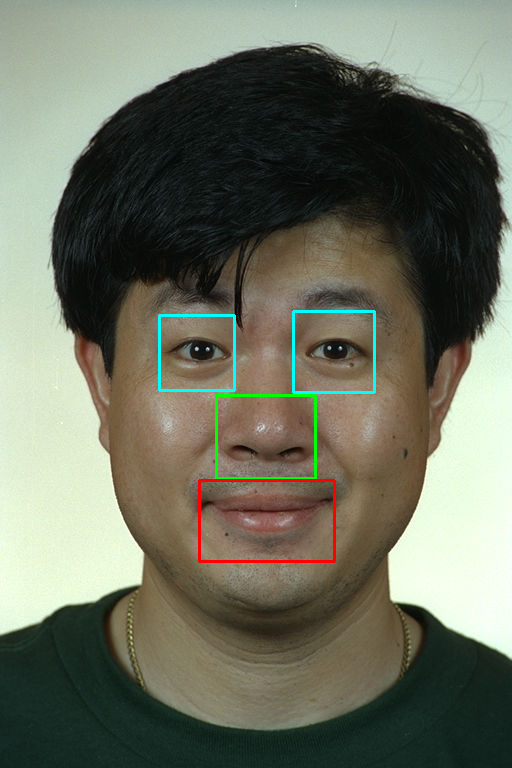
\includegraphics[width=0.9\linewidth]{fig/02_detected_features.png}
        \legend{2º Detecção das características.}
        \label{fig:caracteristicas}
    \end{minipage}
    \label{fig:deteccao-caracteristicas}
\end{figure}



\section{Extração de Contornos}

A detecção de bordas é essencial para a análise de imagens, pois permite a identificação de contornos e a segmentação de objetos em uma cena. O algoritmo \cite{Canny} é um dos métodos mais populares devido à sua eficiência e precisão. Esta parte irá explorar o funcionamento do algoritmo de Canny e demonstrará sua aplicação prática com a biblioteca OpenCV \cite{CannyAplicacao}.

\subsection{Algoritmo de Canny}

O algoritmo de detecção de bordas de Canny é composto por várias etapas, conforme descrito a seguir:

\begin{enumerate}
    \item \textbf{Redução de Ruído}: A imagem é suavizada com um filtro Gaussiano para minimizar a interferência do ruído na detecção de bordas.

    \item \textbf{Cálculo do Gradiente de Intensidade}: Os gradientes de intensidade são calculados nas direções horizontal \(G_x\) e vertical \(G_y\) usando operadores Sobel. A magnitude do gradiente é dada por:
    \[G_x = \frac{\partial I}{\partial x} \quad G_y = \frac{\partial I}{\partial y}\]
    \[Borda\_Gradiente(G) = \sqrt{G_{x}^{2} + G_{y}^{2}}\]

    \item \textbf{Supressão Não Máxima}: Elimina \textit{pixels} que não são máximos locais no gradiente, preservando apenas os que representam bordas fortes.

    \item \textbf{Rastreamento de Bordas por Histerese}: Classifica as bordas detectadas usando dois limiares, \textit{minVal} e \textit{maxVal}:
    \begin{itemize}
        \item Bordas com gradiente maior que \textit{maxVal} são fortes.
        \item Bordas com gradiente menor que \textit{minVal} são descartadas.
        \item Bordas entre \textit{minVal} e \textit{maxVal} são fracas e mantidas apenas se conectadas a bordas fortes.
    \end{itemize}
\end{enumerate}

Por exemplo, na Figura \autoref{fig:histerese}, a borda A está acima do \textit{maxVal}, sendo assim considerada uma \textit{sure-edge}. Embora a borda C esteja abaixo do \textit{maxVal}, ela está conectada à borda A, de modo que também é considerada como borda válida, resultando em uma curva completa. Já a borda B, embora esteja acima do \textit{minVal}, não está conectada a nenhuma \textit{sure-edge} e, portanto, é descartada.

\imagem{Rastreamento de contorno por histerese}{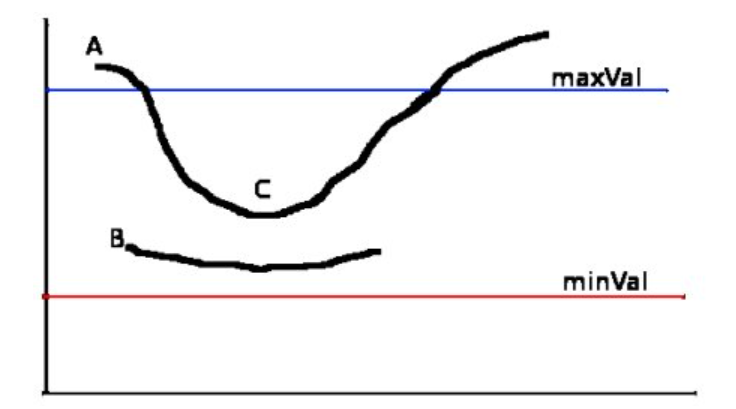
\includegraphics[width = 80mm]{fig/histerese}}{\cite{CannyAplicacao}}{histerese}{}{Calculada a magnitude do gradiente ao longo de uma curva parametrizada.}

É crucial selecionar adequadamente os valores de \textit{minVal} e \textit{maxVal} para obter resultados precisos. Esse estágio também ajuda a remover pequenos ruídos de pixels, assumindo que as bordas são linhas longas e contínuas.

\subsection{Resultado da Detecção de Bordas}
\label{sec:resultado-deteccao-bordas}

Ao aplicar o algoritmo de Canny para a detecção de bordas, obtemos um array binário onde os valores '0' e '255' representam diferentes tipos de pixels. Os pixels com valor '0' são considerados descartáveis, ou seja, não fazem parte das bordas detectadas. Em contraste, os pixels com valor '255' são os que definem as bordas, indicando regiões de mudança de intensidade significativa na imagem original.

A seguir são apresentados os resultados da aplicação do algoritmo de Canny em imagens de exemplo. A \autoref{fig:canny-aplicacao} mostra as características com as bordas detectadas.


\begin{figure}[h!]
    \caption{APLICAÇÃO DO ALGORITMO DE CANNY.}
    \centering
    \begin{minipage}[b]{0.45\textwidth}
        \centering
        
\includegraphics[width=0.9\linewidth]{fig/03_left_eye_edge.png}
        \legend{Olho esquerdo.}
        \label{fig:canny-esquerdo}
    \end{minipage}
    \hfill
    \begin{minipage}[b]{0.45\textwidth}
        \centering
        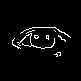
\includegraphics[width=0.9\linewidth]{fig/03_right_eye_edge.png}
        \legend{Olho direito.}
        \label{fig:canny-direito}
    \end{minipage}

    \vspace{1cm}

    \begin{minipage}[b]{0.45\textwidth}
        \centering
        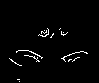
\includegraphics[width=0.9\linewidth]{fig/03_nose_edge.png}
        \legend{Nariz.}
        \label{fig:canny-nariz}
    \end{minipage}
    \hfill
    \begin{minipage}[b]{0.45\textwidth}
        \centering
        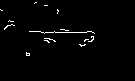
\includegraphics[width=0.9\linewidth]{fig/03_mouth_edge.png}
        \legend{Boca.}
        \label{fig:canny-boca}
    \end{minipage}
    \label{fig:canny-aplicacao}
\end{figure}
% \newpage
A detecção de bordas de Canny é uma técnica poderosa e eficiente para identificar contornos em imagens. Esses resultados demonstram como o algoritmo de Canny é eficaz para realçar as bordas em diferentes tipos de imagens, permitindo uma análise visual clara e detalhada das características principais em cada exemplo.

\newpage

\section{Redução de Pontos em Detecção de Bordas}
\label{sec:reduzindo-pontos-deteccao-bordas}


Embora o detector de bordas de Canny seja excelente para capturar as bordas, nem sempre é necessário utilizar todos os pontos detectados ao passar uma spline. Para a modelagem de contornos suaves e contínuos, é suficiente selecionar um subconjunto representativo dos pontos detectados. Esse processo pode envolver a amostragem ou a simplificação dos pontos de borda, garantindo que a spline mantenha a forma geral do contorno sem a complexidade de lidar com todos os pontos individuais.

Esta parte é realizada em quatro etapas principais:
\begin{enumerate}
    \item \textbf{Construção do Grafo:} Os pontos de borda detectados são organizados em um grafo, onde cada ponto é um nó e as conexões entre eles representam as arestas. Essa estrutura facilita a análise e a manipulação dos pontos.
    \item \textbf{Árvore Geradora Mínima:} A partir do grafo, uma árvore geradora mínima é construída. Essa árvore conecta todos os pontos de forma a minimizar o custo total das arestas, resultando em uma representação simplificada dos contornos.
    \item \textbf{Otimização com Poda da Árvore:} A árvore geradora mínima é otimizada, removendo pontos que não contribuem significativamente para a forma geral do contorno. Essa poda reduz o número de pontos, mantendo apenas os mais relevantes.
    \item \textbf{Filtragem Aleatória:} Por fim, uma filtragem aleatória é aplicada para suavizar ainda mais a representação, mantendo apenas os pontos iniciais e finais de cada segmento. Essa etapa garante que a spline resultante seja suave e contínua.
\end{enumerate}

\subsection{Grafos}

Para a construção do grafo, utilizamos os pontos de borda detectados pelo algoritmo de Canny. Cada ponto é representado como um nó no grafo, e as conexões entre os nós são representadas como arestas. Essa estrutura é chamada de matriz de adjacência, onde cada elemento indica a presença ou ausência de uma aresta entre dois nós.

O código foi feito de forma autoral em Python, utilizando a fórmula Manhattan para calcular a distância entre os nós. Essa fórmula é adequada para o nosso caso, pois considera apenas as distâncias horizontais e verticais, o que é suficiente para que o grafo represente adequadamente a estrutura dos contornos faciais.

No processo de detecção de contornos, a matriz Canny e a matriz de adjacências são conceitos fundamentais para entender a construção dos grafos. O primeiro passo é aplicar a matriz Canny, que resulta na detecção de contornos da imagem. A seguir, apresentamos uma representação da matriz Canny e da matriz de adjacências.

\begin{figure}[ht]
    \caption{MATRIZ CANNY E CONTORNOS.}
    \label{fig:canny-contornos}
    \centering
    \begin{tabular}{c c c}
        \begin{minipage}{0.4\textwidth}
            \centering
            \textbf{Matriz Canny}\\ [0.2cm]
            \[
            \begin{bmatrix}
                255_1 & 0 & 0 & 0 & 0 \\
                0 & 255_2 & 0 & 255_3 & 0 \\
                255_4 & 0 & 0 & 0 & 255_5 \\
            \end{bmatrix}
            \]
        \end{minipage}
        \hspace{0.5cm}
        
        & $\rightarrow$ &
        \begin{minipage}{0.4\textwidth}
            \centering
            \textbf{Contornos}\\ [0.2cm]
            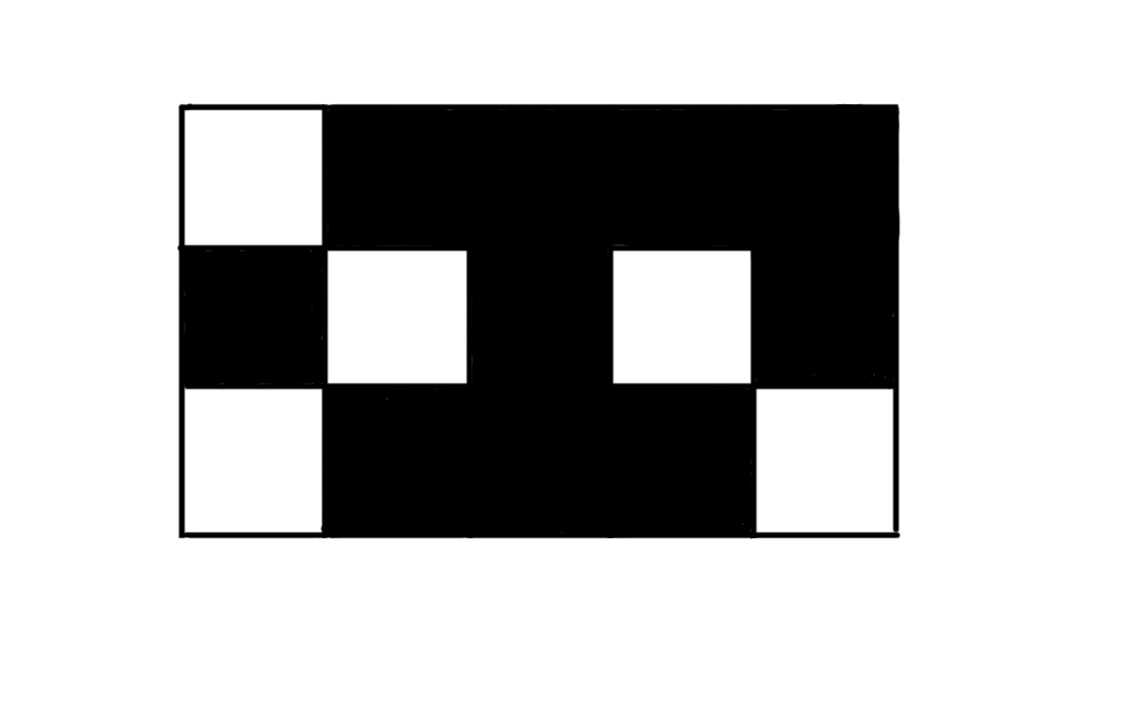
\includegraphics[width=0.9\textwidth]{fig/contorno_canny.jpeg}
        \end{minipage}
    \end{tabular}
    \end{figure}

O próximo passo é a conversão dos contornos em grafos utilizando a matriz de adjacências.

\begin{figure}[ht]
    \caption{MATRIZ DE ADJACÊNCIAS E GRAFO.}
    \label{fig:adjacencias-grafo}
    \centering
    \begin{tabular}{c c c}
        \begin{minipage}{0.4\textwidth}
            \textbf{Matriz de Adjacências}\\[0.2cm]
            \centering
            \[
            \begin{bmatrix}
                0 & 1 & 0 & 0 & 0 \\
                1 & 0 & 0 & 1 & 0 \\
                0 & 0 & 0 & 0 & 1 \\
                0 & 1 & 0 & 0 & 0 \\
                0 & 0 & 1 & 0 & 0 \\
            \end{bmatrix}
            \]
        \end{minipage}
        \hspace{0.5cm}
        
        & $\rightarrow$ &
        \begin{minipage}{0.4\textwidth}
            \centering
            \textbf{Grafo}\\[0.2cm]
                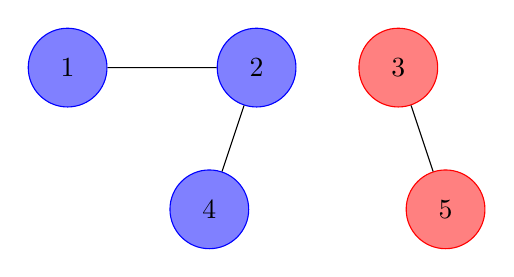
\begin{tikzpicture}[scale=1.2, every node/.style={circle, draw, minimum size=1cm}]
                    % Triângulo
                    \node [fill = blue!50, draw = blue] (1) at (2,1.5) {1};
                    \node [fill = blue!50, draw = blue] (2) at (4,1.5) {2};
                    \node [fill = blue!50, draw = blue] (4) at (3.5,0) {4};
                
                    % Conexão do nó 1 com nó 5 ao lado
                    \node [fill = red!50, draw = red](3) at (5.5, 1.5) {3};
                    \node [fill = red!50, draw = red](5) at (6,0) {5};
                
                    \draw (1) -- (2) -- (4);
                    \draw (3) -- (5);
                \end{tikzpicture}
        \end{minipage}
    \end{tabular}
    \end{figure}

\newpage

\subsection{Grafos Conexos e Desconexos}

Os grafos podem ser classificados em dois tipos principais: grafos conexos e grafos desconexos. Um grafo é considerado conexo se existe pelo menos um caminho entre qualquer par de nós do grafo. Por outro lado, um grafo desconexo possui pelo menos um par de nós que não estão conectados por um caminho.

Um grafo desconexo pode ser dividido em componentes conexos, que são subgrafos conexos. Cada componente conexo é um subconjunto do grafo original onde todos os nós estão conectados entre si, mas não há conexão com os nós de outros componentes. Essa distinção é importante para entender a estrutura do grafo e como ele pode ser analisado e manipulado.


\begin{figure}[ht]
    \caption{COMPONENTES CONEXOS REPRESENTADAS POR GRAFOS.}
    \centering
    \begin{minipage}{0.45\textwidth}
        \centering
        \textbf{Componente Conexo 1} \\[0.2cm]
        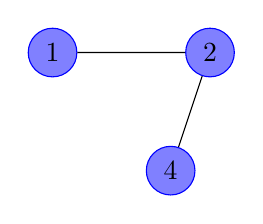
\begin{tikzpicture}
            % Primeiro grafo (Triângulo) - Cor Azul
            \node at (2,1.5) (n1) [circle, draw=blue, fill=blue!50] {1};
            \node at (4,1.5) (n2) [circle, draw=blue, fill=blue!50] {2};
            \node at (3.5,0) (n3) [circle, draw=blue, fill=blue!50] {4};
            \draw (n1) -- (n2) -- (n3);
            % \draw (n2) -- (n3);
            % \draw (n3) -- (n1);
        \end{tikzpicture}
    \end{minipage}
    \hfill
    \begin{minipage}{0.45\textwidth}
        \centering
        \textbf{Componente Conexo 2} \\[0.2cm]
        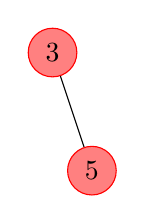
\begin{tikzpicture}
            % Segundo grafo (Quadrado) - Cor Vermelha
            \node at (1.5,1.5) (n1) [circle, draw=red, fill=red!50] {3};
            \node at (2,0) (n2) [circle, draw=red, fill=red!50] {5};
            % \node at (2,2) (n3) [circle, draw=red, fill=red!50] {6};
            % \node at (0,2) (n4) [circle, draw=red, fill=red!50] {7};
            \draw (n1) -- (n2);
            % \draw (n2) -- (n3);
            % \draw (n3) -- (n4);
            % \draw (n4) -- (n1);
        \end{tikzpicture}
    \end{minipage}
    \label{fig:componentes_conexos}
    \end{figure}

Em problemas de processamento de imagens, frequentemente são utilizados grafos que representam os pixels da imagem. O objetivo é identificar componentes conexos, permitindo a seleção dos caminhos mais significativos e a filtragem de ruídos. Componentes com um grande número de nós indicam regiões de interesse, correspondendo a áreas com maior quantidade de pixels conectados. Por outro lado, componentes menores podem ser interpretadas como ruído ou regiões irrelevantes, que podem ser descartadas durante o processamento.

\subsection{Resultado da Construção do Grafo}
\label{sec:resultado-construcao-grafo}

Podemos observar que a imagem original é composta por um grande número de pontos, porém utilizando a filtragem de pixels através de grafos com as componentes conexos, conseguimos reduzir a quantidade de pontos, mantendo apenas os mais relevantes. A \autoref{fig:resultado-grafo} mostra o resultado da construção do grafo e a filtragem dos pontos.

\begin{figure}[h!]
    \caption{COMPONENTES CONEXOS OLHO DIREITO.}
    \centering
    \begin{minipage}[b]{0.45\textwidth}
        \centering
        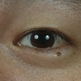
\includegraphics[width=0.9\linewidth]{fig/02_detected_right_eye.png}
        \legend{Olho direito identificado.}
        \label{fig:olho}
    \end{minipage}
    \hfill
    \begin{minipage}[b]{0.45\textwidth}
        \centering
        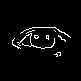
\includegraphics[width=0.9\linewidth]{fig/03_right_eye_edge.png}
        \legend{Ênfase nos contornos.}
        \label{fig:canny-olho}
    \end{minipage}

    \vspace{1cm}

    \begin{minipage}[b]{0.45\textwidth}
        \centering
        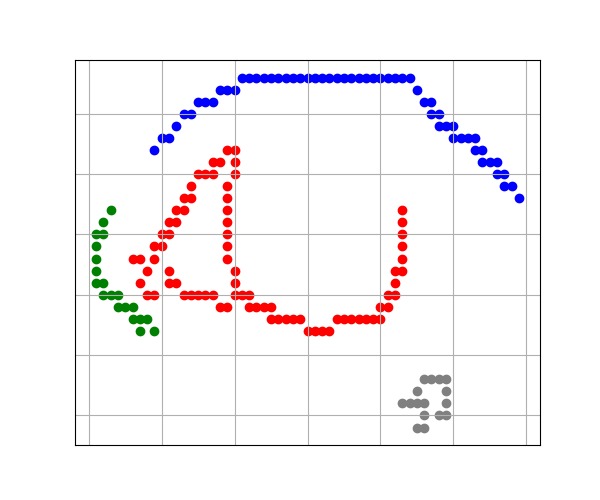
\includegraphics[width=1\linewidth]{fig/04_connected_components_right_eye.png}
        \legend{Remoção de alguns pontos através dos maiores compenentes conexos.}
        \label{fig:grafos-olho}
    \end{minipage}
    \label{fig:resultado-grafo}
\end{figure}

\subsection{Árvore Geradora Mínima}
\label{sec:arvore-geradora-minima}

A árvore geradora mínima (AGM) é uma estrutura de dados fundamental em teoria dos grafos, que conecta todos os nós de um grafo com o menor custo total possível. Essa estrutura é especialmente útil em aplicações de processamento de imagens, onde a simplificação de contornos e a redução do número de pontos são necessárias para facilitar a modelagem e a análise. Neste trabalho foi utilizada a biblioteca \textit{Scipy} \cite{Scipy} para encontrar a AGM.

Cada nó na AGM tem uma relação hierárquica com outros nós:

\begin{itemize}
    \item O nó raiz é o nó inicial a partir do qual a árvore é construída ou percorrida.
    \item Um nó filho é aquele que se origina de outro nó — chamado de pai — seguindo essa ideia de crescimento ou expansão da árvore.
    \item É um nó que não tem filhos, ou seja, ele está no fim de um caminho na árvore
\end{itemize}


Para a construção adequada das splines, é essencial definir uma ordem consistente para os pontos que descrevem as características faciais. Sem uma ordem definida, as splines podem ser traçadas de maneira incoerente, resultando em representações visuais incorretas ou deformadas. Além disso, a ordenação contribui para evitar ciclos ou conexões redundantes entre os pontos, o que poderia comprometer a suavidade e continuidade das curvas. Foi utilizada a biblioteca \textit{Scipy} \cite{Scipy} para encontrar a AGM.

Para otimizar a análise, aplicamos uma \textbf{poda da árvore} na AGM para identificar o caminho principal e eliminar os pontos que não contribuem significativamente para a forma geral do contorno. Essa poda é realizada com base em critérios de distância e relevância, garantindo que apenas os pontos mais significativos sejam mantidos na representação final.

% O algoritmo para a otimização da árvore encontrando o maior caminho foi feito de forma autoral em Python, foi construído da seguinte forma:

Veja abaixo a implementação do método \texttt{prunning\_tree}. Ele percorre recursivamente a árvore para calcular a altura dos nós e determinar o caminho de maior comprimento entre dois nós folha.

\begin{lstlisting}[language=Python, caption={IMPLEMENTAÇÃO DO MÉTODO \texttt{prunning\_tree}.}, label={lst:prunning_tree}]
def prunning_tree(self, raiz):
    # Se o nó atual não tem filhos, é uma folha
    if len(raiz.filhos) == 0:
        return 1, [raiz.idx], 1, [raiz.idx]
    else:
        # Para cada filho, executa a função recursivamente
        for filho in raiz.filhos:
            filho.altura, filho.caminho_altura_maxima, filho.tamanho_caminho_maximo, filho.caminho_maximo = self.prunning_tree(filho)

        if len(raiz.filhos) == 1:
            # Verifica se o caminho que passa pelo nó atual é maior que o maior caminho encontrado até o momento
            if raiz.filhos[0].altura + 1 > raiz.filhos[0].tamanho_caminho_maximo:
                tamanho_caminho_maximo = raiz.filhos[0].altura + 1
                caminho_maximo = [raiz.idx] + raiz.filhos[0].caminho_altura_maxima
            else:
                # Usa o maior caminho já encontrado no filho
                tamanho_caminho_maximo = raiz.filhos[0].tamanho_caminho_maximo
                caminho_maximo = raiz.filhos[0].caminho_maximo
        else:
            # Ordena os filhos pela altura (do maior para o menor)
            raiz.filhos.sort(key=lambda x: x.altura, reverse=True)

            # Calcula o maior caminho passando por este nó (soma das duas maiores alturas + o nó atual)
            tamanho_caminho_maximo = raiz.filhos[0].altura + raiz.filhos[1].altura + 1

            # Monta o caminho correspondente
            uma_parte_do_caminho = raiz.filhos[0].caminho_altura_maxima.copy()
            uma_parte_do_caminho.reverse()
            caminho_maximo = uma_parte_do_caminho + [raiz.idx] + raiz.filhos[1].caminho_altura_maxima

            # Verifica se algum filho tem um caminho maior do que esse
            for filho in raiz.filhos:
                if filho.tamanho_caminho_maximo > tamanho_caminho_maximo:
                    tamanho_caminho_maximo = filho.tamanho_caminho_maximo
                    caminho_maximo = filho.caminho_maximo

        # Pega o filho com maior altura (o primeiro da lista, já ordenada)
        no_altura_maxima = raiz.filhos[0]

        return no_altura_maxima.altura + 1, [raiz.idx] + no_altura_maxima.caminho_altura_maxima, tamanho_caminho_maximo, caminho_maximo

\end{lstlisting}

O funcionamento do algoritmo pode ser resumido nos seguintes passos:

\begin{enumerate}
    \item \textbf{Calculando a Altura da Árvore} medindo a profundidade máxima a partir da raiz até as folhas.
    \item \textbf{Calculando o Maior Caminho} dentro dos nós da árvore.
    \item O maior desses dois valores é considerado o \textbf{caminho principal}, capturando a estrutura mais relevante e eliminando nós de menor importância.
\end{enumerate}


\begin{figure}[ht]
    \centering
    \caption{PODA DA AGM.}
    \label{fig:poda-arvore-geradora-minima}
    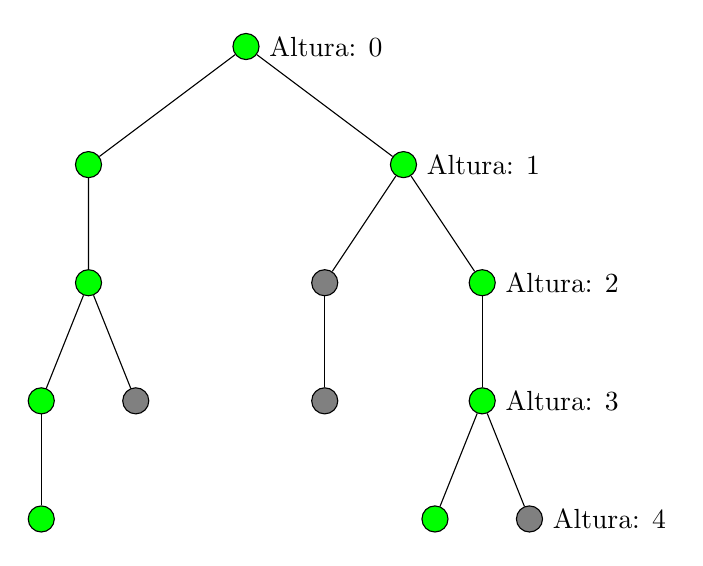
\begin{tikzpicture}[
      level distance=1.5cm,
      level 1/.style={sibling distance=4cm},
      level 2/.style={sibling distance=2cm},
      level 3/.style={sibling distance=1.2cm}
      ]
    
    \node[circle, draw, fill= green, label=right:{Altura: 0}] {} 
      child {node[circle, draw, fill = green] {} 
        child {node[circle, draw, fill = green] {}
          child {node[circle, draw, fill = green] {}
            child {node[circle, draw, fill = green] {}}
          }
          child {node[circle, draw, fill = gray] {}}
        }
      }
      child {node[circle, draw, fill = green, label=right:{Altura: 1}] {}
        child {node[circle, draw, fill = gray] {}
          child {node[circle, draw, fill = gray] {}}
        }
        child{node[circle, draw, fill = green, label=right:{Altura: 2}] {}
          child {node[circle, draw, fill = green, label=right:{Altura: 3}] {}
            child {node[circle, draw, fill = green] {}}
            child {node[circle, draw, fill = gray, label=right:{Altura: 4}] {}}
          }
        }
      };
    
    \end{tikzpicture}
    \legend{LEGENDA: Em verde: nós que fazem parte do maior caminho. Em cinza: nós que não fazem parte do maior caminho.}
\end{figure}

Pela \autoref{fig:poda-arvore-geradora-minima} podemos observar como funciona o algoritmo que realiza a poda da AGM, mantendo apenas os nós que fazem parte do maior caminho. Esta etapa é essencial para simplificar a representação dos contornos e facilitar a modelagem das \textit{splines}.

\subsection{Resultado da AGM}
\label{sec:resultado-agm}

A \autoref{fig:resultado-agm} mostra o resultado da AGM, onde os pontos que não fazem parte do maior caminho foram removidos e logo após a AGM, aplicamos mais um algoritmo autoral que elimina pontos de forma aleatória, mantendo apenas os pontos iniciais e finais de cada segmento.

\begin{figure}[h!]
    \caption{FILTRAGEM DE PONTOS PELA AGM.}
    \centering
    \begin{minipage}[b]{0.45\textwidth}
        \centering
        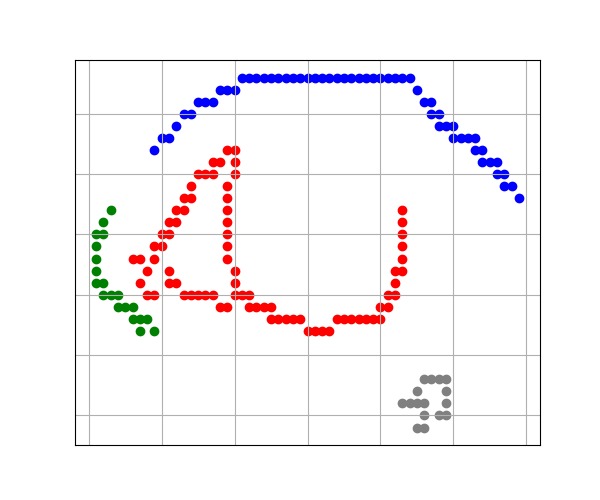
\includegraphics[width=0.9\linewidth]{fig/04_connected_components_right_eye.png}
        \legend{Maiores componentes conexos.}
        \label{fig:olho-grafo}
    \end{minipage}
    \hfill
    \begin{minipage}[b]{0.45\textwidth}
        \centering
        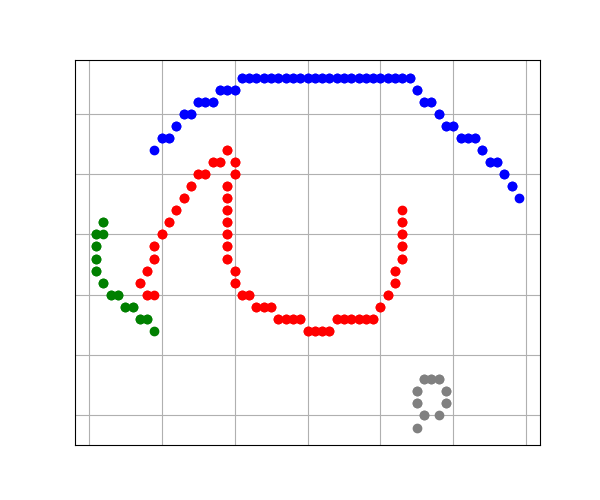
\includegraphics[width=0.9\linewidth]{fig/05_longest_path_right_eye.png}
        \legend{Aplicação da poda da AGM.}
        \label{fig:olho-agm}
    \end{minipage}

    \vspace{1cm}

    \begin{minipage}[b]{0.45\textwidth}
        \centering
        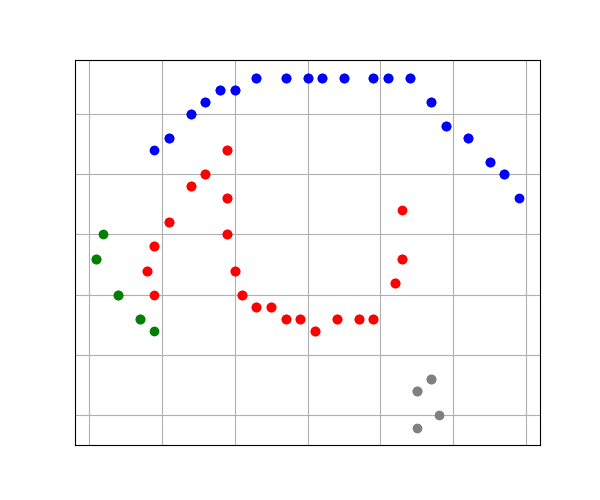
\includegraphics[width=1\linewidth]{fig/06_new_longest_path_right_eye.png}
        \legend{Remoção de alguns pontos de forma aleatória.}
        \label{fig:olho-aleatorio}
    \end{minipage}
    \label{fig:resultado-agm}
\end{figure}


%%% explicar melhor porque estamos usando a AGM: ordem para a construção da spline, evitar ciclos, etc.